\chapter[Introduction]{Introduction}\label{chap_intro}

\section{Motivation}
\label{Sec:Motivation}

Recent works \cite{Ghanta022019, Crankshaw2017, Polyzotis2018}, highlight some of the challenges encountered in spatio-temporal predictive serving systems. In such systems, values of variables whose behavior varies in space-time are inferred by predictive models built over regions of the spatio-temporal domain. In this context, we are interested in the problem arising in the presence of multiple competing predictive models, i.e., models that predict the same variable but are built independently over potentially different regions of the domain. It may be the case in large companies where autonomously developed models about the same phenomenon (a.k.a. competing models) are deployed and used to answer predictive queries. 

A predictive serving system enables users to express queries that specify: a spatio-temporal region, a target variable, and an evaluation metric. The outcome of the query presents the target variable's values on the specified region computed by predictive models that maximize the evaluation metric. 

However, identifying the  models to be used by the system to answer the predictive query is a hard problem. It is due to the fact that competing  models present varying predictive behavior through regions of the domain. It may be due to learners' intrinsic learning capabilities and variations on spatio-temporal regions used to construct independently built models. In this context, our goal is to define a procedure that selects a set of models that computes the query answer and maximizes the evaluation metric, see Figure \ref{Fig:MotiPoster}. 

\begin{figure}[h]
	\centering
	\includegraphics[scale=0.3]{../Figures/ModelManagementPS-VersionCompleta}
	\caption{Predictive Serving System Models.}
	\label{Fig:MotiPoster}
	%	\Description{ML Model Lifecycle.}
\end{figure}

Our approach objective is to quantify the predictive quality for auto-regressive models using a shape-based characterization of the domain. In particular, we compute the data distribution on regions of the domain where the models have been trained and compare them against those within the query spatio-temporal region. The intuition is that model behavior in query regions with similar data distribution as the ones used to train the model shall follow the one observed during training. Conversely, in spatio-temporal regions specified by the query and that have not been used for training, the model would exhibit an error computed as a function of the distance between the query non seen data region and the model building data region.

\subsection{Problem Statement}
\label{Sec:ProblemStatement}

Given a phenomenon with a spatio-temporal domain, represented by univariate time series, where independent predictive models have been trained, select a model or a composition of models to answer a spatio-temporal predictive query that maximizes an evaluation metric.

\section{Objective and Contribution}
\label{Sec:ObjectiveContribution}
\Fab{Precisa colocar claramente o objetivo da tese. Exemplo: The objective of this theses is to propose a new method to allocate time-series models to a spatio-temporal data region such that their predictions optimize a specified prediction metric".}

(TODO) Our approach aims to quantify the predictive quality of models by characterizing patterns within the predictive variable domain data. In particular, we identify some patterns on domain regions where the models have been trained and compare them against patterns within the query spatio-temporal region. Our hypothesis is that if a query region has similar data patterns as the regions used to train the model, then the behavior of the model on the query region should follow the one observed during training.
Conversely, in spatio-temporal regions specified by the query that have not been used for training, the model would exhibit an error computed as a function of the distance between the query non seen data region and the model building data region.
\Fab{O proximo paragrafo parece um tanto perdido na seção}
A collection of time series can exhibit various dependency relationships between the individual time series that can be leveraged in forecasting. It includes:
(i) local co-variate relationships (e.g., the price and demand for a product, which tend to be (negatively) correlated),
(ii) indirect relationships through shared latent causes (e.g., demand for multiple products increasing because an advertising campaign is driving traffic to the site),
(iii) subtle dependencies through smoothness, temporal dynamics, and noise characteristics of time series measurements of similar underlying phenomena (e.g., product sales time series tend to be similar to each other but different from energy consumption time series).
The data in practical forecasting problems typically have all of these forms of dependencies. Using this data from related time series allows more complex and potentially more accurate models to be fitted without overfitting.
\Fab{Achei que faltou um exemplo de aplicação materializando a motivação. O capitulo ficou meio no ar. De onde saiu este problema? Que caracteristicas ele aprsenta? O que ja foi feito na literatura e a lacuna que se quer preencher?}

\section{Problem Formalization}
\label{Sec:ProblemFormalization}

Let $\mathcal{D} = \{(\mathcal{S},( x, y)): \,\, \mathcal{S} = \{s_{1}, s_{2}, \ldots, s_{t}\}$ is a univariate time-series, and $(x,y) \in \mathbb{R}^{2}\}$, represents a spatio-temporal domain. Denote by $\mathcal{G} = \{g_{1}, g_{2}, \ldots \}$ the set of temporal predictive models that were trained for different subsets $\mathbf{S} \subseteq \mathcal{D}$. Each predictive model $g\in \mathcal{G}$ is denoted as follows:
\begin{equation}
\label{eq:ModelDefinition}
g = \langle \mathbf{S}, A, \mathbf{p}, E, \varSigma \rangle,
\end{equation}
where:
\begin{itemize}[noitemsep,nolistsep]	
	\item $\mathbf{S}$: input dataset included in the spatio-temporal domain $\mathcal{D}$,
	\item $A$: learner or hypothesis set,
	\item $\mathbf{p}$: model parameters (number of time-units to obtain the in-sample error ($t_{p}$), number of time-units to forecast ($t_{f}$)),
	% REVIEW !!!
	\item $E$: in-sample error (generally computed by the difference between the predicted value by $g$ and the actual value in the dataset),
	\item $\varSigma$: implementation/execution quality metrics.
\end{itemize}

% Models for a regions and discrete regions that coulld be characterized by an element, we assume that the element leads to a predictive model, capable of predict elements of its region with high accuracy (inside some threshold). 
In this context, given a predictive spatio-temporal query $Q$ denoted as:
\begin{equation} \label{eq:predictivequery}
Q = \langle R, t_{p}, t_{f}, Q_{m} \rangle,
\end{equation}
where:
\begin{itemize}[noitemsep,nolistsep]	
	\item $R$: represents the size/shape/type of interest region,
	\item $t_{p}$: $\{s_{t-t_p}, s_{t-t_{p}+1}\ldots, s_{t}\}$ number of steps used for  prediction,
	\item $t_{f}$: $\{s_{t+1}, \ldots, s_{t+t_f}\}$ number of steps to predict ($n\geq 1$),
	\item $Q_{m}$: represents users qualitative measurements to evaluate the predictive output.
\end{itemize}

% We are interested in attend or process this query with this handful of models in a way that guarantee a degree of accuracy.

We formally define our problem: Let the spatio-temporal domain characterization $\mathcal{D} = \bigcup_{i=1}^{n} \mathbf{S_i}$ and $\mathcal{G}$ the set of temporal models for a single element of $\mathbf{S_i}$ that accounts for the in-sample error bounds for the elements in $\mathbf{S_i}$. Given $Q = \langle R, t_{p}, t_{f}, Q_{m} \rangle$:

\begin{equation}
\forall \mathcal{S} \in R: \exists g \in \mathcal{G'} \,\,\textrm{such that} \,\, \argminA_{g\in\mathcal{G'}} E_{g}(R).
\end{equation}

%TODO Change the argmin 
\noindent In Figure \ref{fig:time-series}, we show the elements involved in the formalization of our problem:
\begin{figure}[htb]
	\centering
	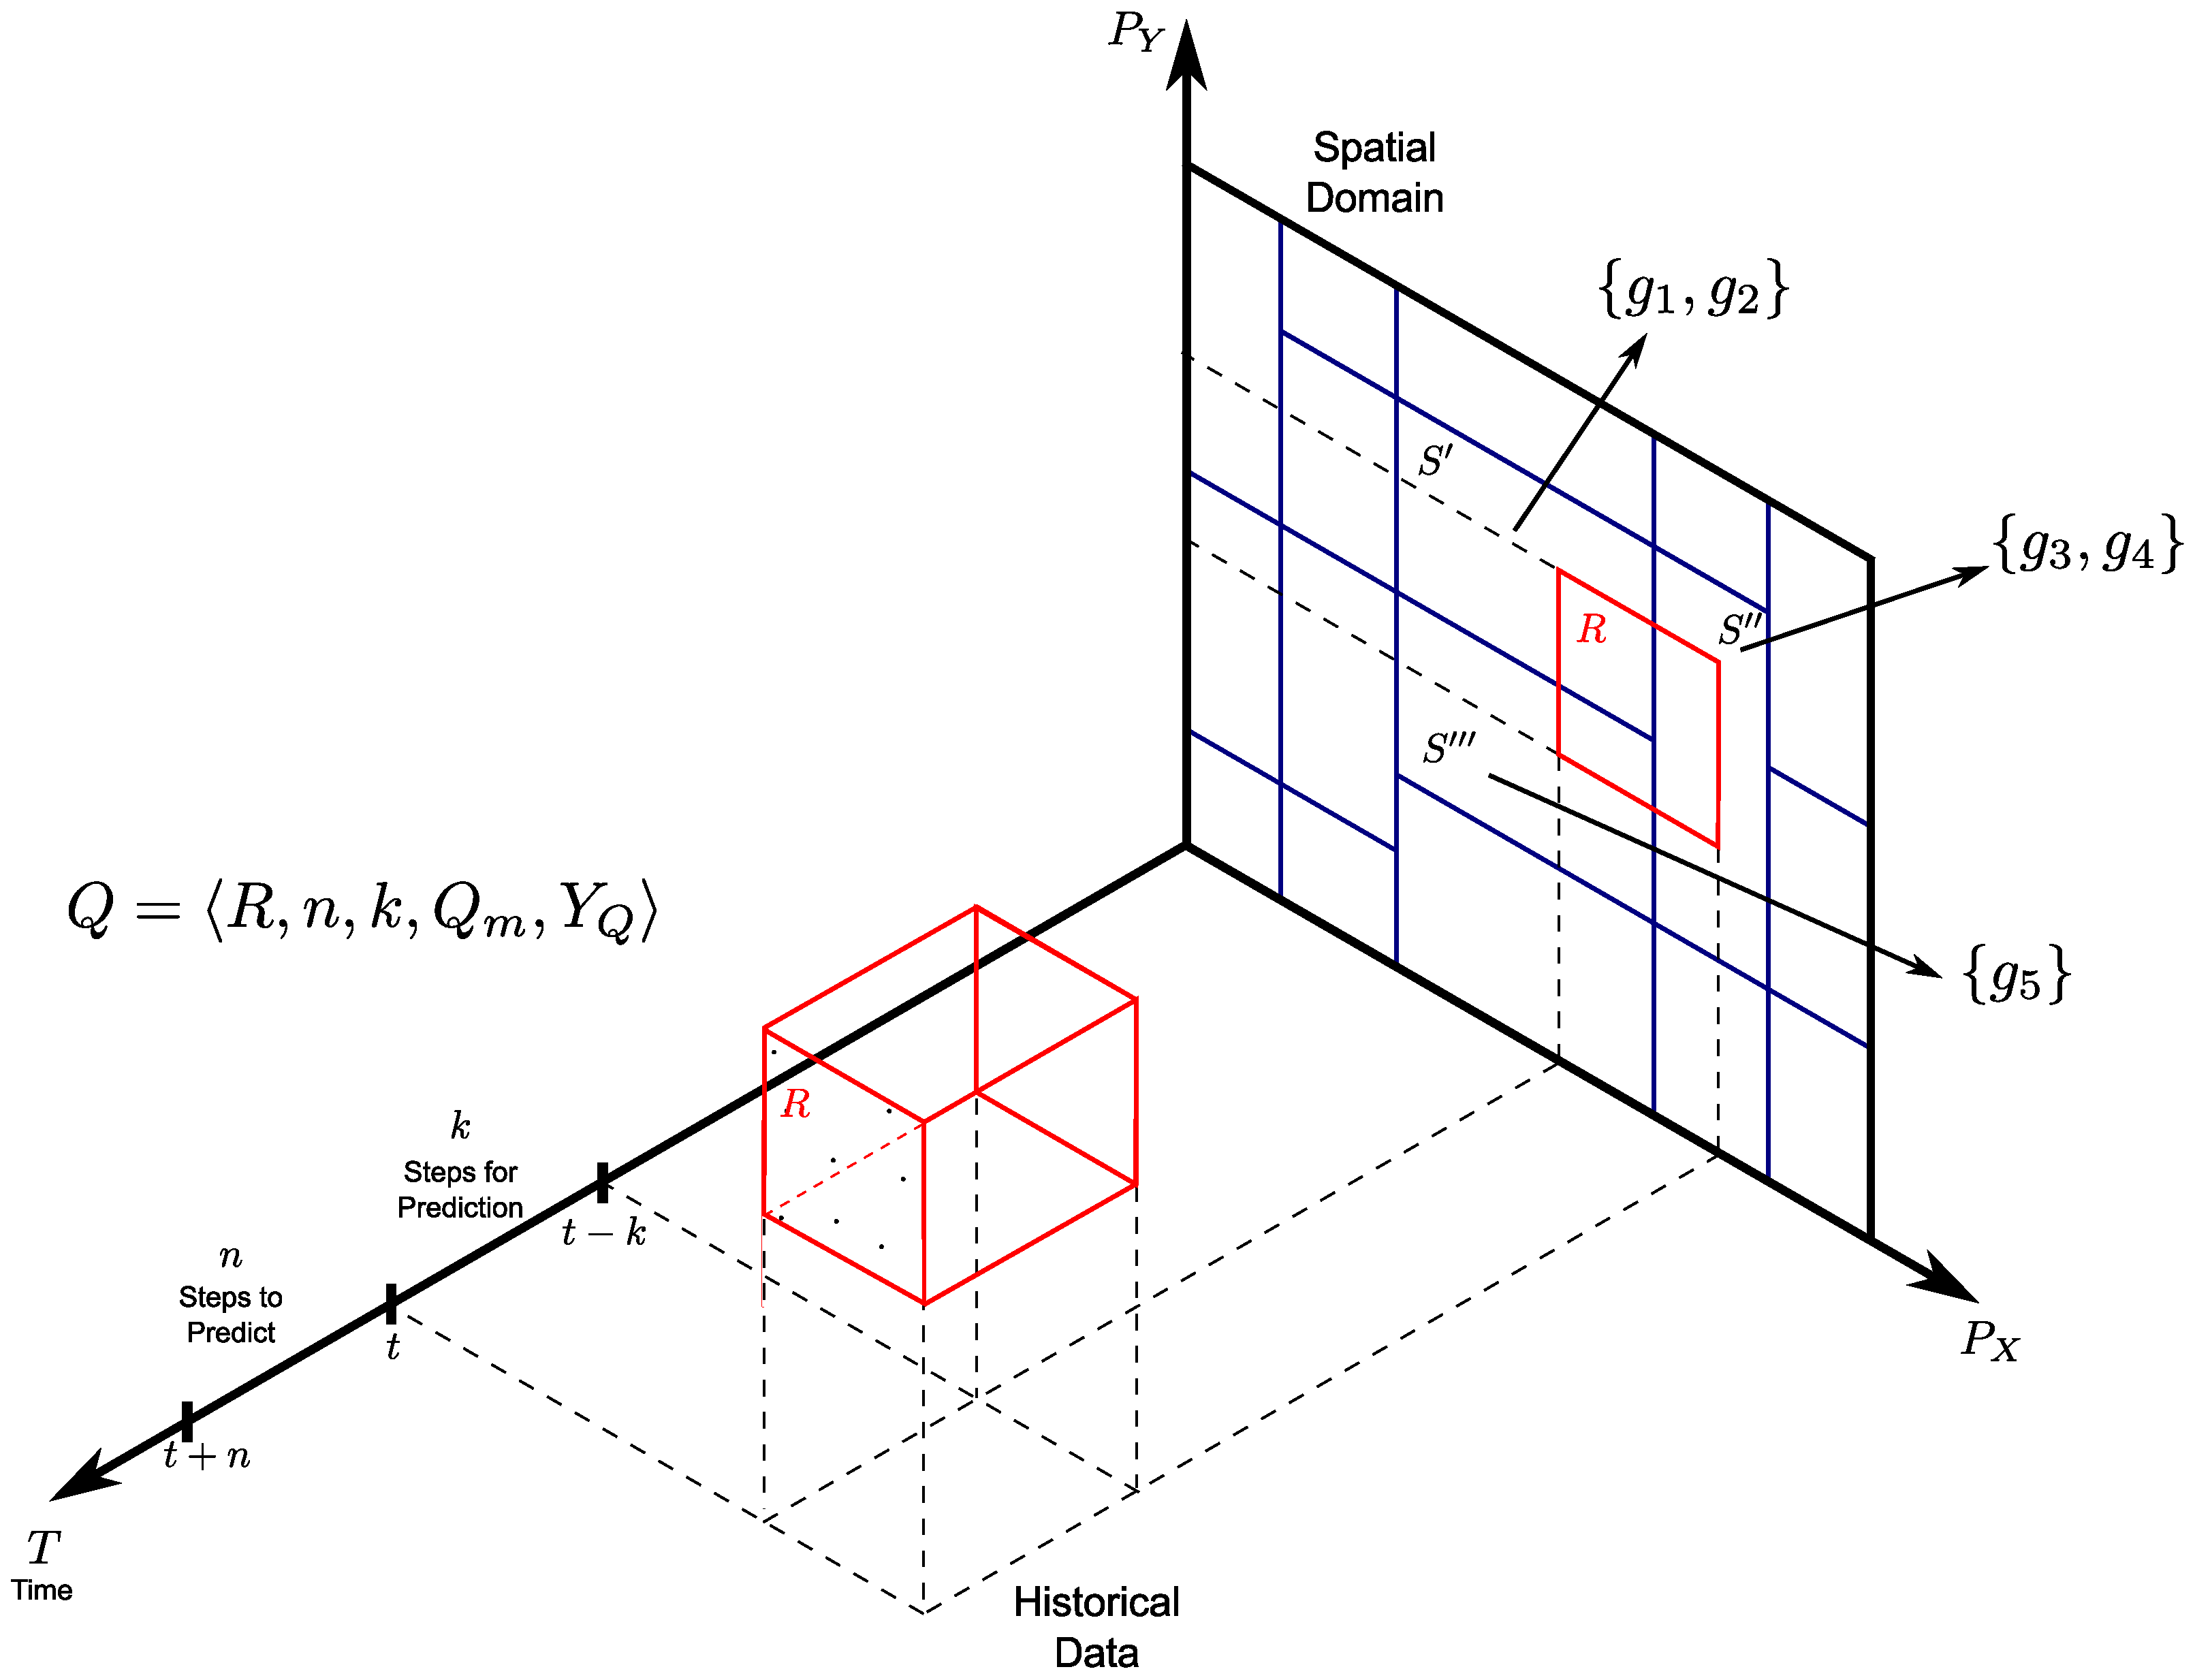
\includegraphics[scale=0.25]{../Figures/RepresentationTimeSeries}
	\caption{Predictive Spatio-Temporal Queries.}
	\label{fig:time-series}
\end{figure}


\section{Thesis Outline}
\label{Sec:ThesisOutline}

The structure of the remainder of this thesis is outlined for reference.

\begin{description}
\item[Chapter 2.] \textbf{[Theoretical Foundations.]} Presents the fundamental approaches of methods and techniques for the task of univariate time series clustering, using shape-based similarity in particular. It is followed by the foundations of neural network approaches for the task of univariate time series classification. Finally, we consider the foundations for time series analysis, with a focus on auto-regressive methods.

\item[Chapter 3.] \textbf{[Related Works.]} Covers a review for other works found in the literature that use similar methods and techniques utilized in our proposed methodology. We include some comparisons that help put our contributions into context. %into  proved to be efficient and 

\item[Chapter 4.] \textbf{[Methodology.]} This chapter is dedicated to elaborating the methodology proposed in this work, providing justifications for some of the decisions made and establishing hypotheses that can be later validated via experiments.

\item[Chapter 5.] \textbf{[Spatio Temporal Tool for Time Series Analysis.]} Describes some architectural aspects of an application designed to implement the proposed methodology and perform the experiments to validate our proposal.

\item[Chapter 6.] \textbf{[Experimental Results.]} Describes the experimental evaluation of the methodology, considering a case study of temperature forecasting. The experiments are organized according to the steps considered in the methodology; for each step, we perform extensive analyses and discuss the results obtained. 

\item[Chapter 7.] \textbf{[Conclusions and Future Works.]} Finally, in this chapter, the main contributions of the thesis are highlighted, and we indicate some future directions for research based on this work.

\end{description}


% TODO move this to intro text
%Formed by an off-line and on-line phase, in this chapter we describe the procedures for: i) a procedure for domain partitioning in order to represent the domain by a set of representatives; ii) the process of generate predictive models for these representatives; iii) a multi class classification approach to select a model to predict a region of interest; and finally iv) the process involved in the execution of a spatiotemporal predictive query. 


% TODO Include in the Introduction
% A hypothesis we want to highlight is that it should be preferable to use a partitioning technique that considers grouping domain elements based on the similarity of their temporal evolution, rather than creating groups just according to a regular division of the domain geometry. To verify this, we compare the intra-cluster sum of both partitioning techniques for several values of $k$.